\documentclass[designspec/spec.tex]{subfiles}

%Sammanfattningen bör innehålla:
%
%   -En beskrivning av de mest framträdande egenskaperna hos det totala
%   systemet och de olika delsystemen.
%
%   -Ett blockschema som beskriver konstruktionens uppdelning i olika delar.
%
%   -En beskrivning av vilka sensorer som ska användas och hur de ska placeras.
%
%   -En beskrivning av vilka ställdon (motorer etc,) som ska användas och hur
%   de ska användas och hur de ska placeras.

\begin{document}

\section{Översikt}
I denna del förklaras designen av systemet översiktligt.

\subsection{Framträdande egenskaper}
Produkten består av tre moduler: Kommunikation-, sensor- och styrmodul.
Sensormodulen kommer implenteras på ett virkort varav de andra modulerna ska
vara på ett separat virkort. Produkten har två avståndsmätare och kamera till
hjälp när produkten ska samla in information om sin omgivning. Vardera
mikrokontroller klockas med en kristalloscillator.

\subsubsection{Fjärrstyrning}
Produkten kopplas till en mobils eller laptops hotspot och fjärrstyrningen sker
via WiFi.

\begin{figure}[h]
    \centering
    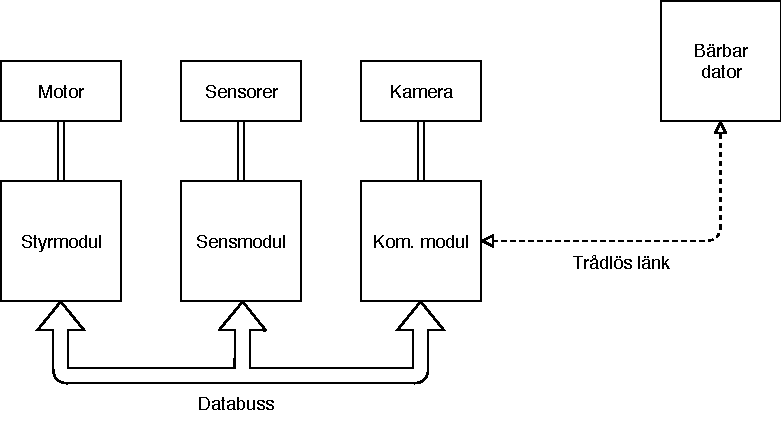
\includegraphics[width=0.6\linewidth]{designspec/fig/blockskiss.pdf}
    \caption{Övergripande bild över systemet och dess moduler. SPI-buss används}
    \label{fig:overview}
\end{figure}

Kommunikationsmodulen består av en raspberry Pi och kommer vara en central
kommunikation- och beslutsenhet som ansvarar för att ta beslut om reglering samt
så sköter den kommunikationen mellan modulerna. Styrmodulen består av motor och
mikrokontroller och står för drift samt regleringen. Sensormodulen består av
mikrokontroller samt avståndsmätare och halleffektsensorn.

\subsection{Placering av sensorer}
Kameran ska fästas en bit ovan alla korten och titta framåt med en vinkel nedåt.
Avståndsmätaren(GP2Y0A02YK) som ska mäta avstånd till hinder ska fästas på
framsidan av bilens chassi. Om det behövs så ska lämpliga fotfästen skrivas ut i
3D-skrivaren. Den andra avståndsmätaren(GP2D120) som används för att mäta ifall
vi har åkt förbi hindret vid omkörning kommer placeras på bakrehöger sida av
bilens chassi. Odometern(Halleffektssensorn) som används till att mäta distans
körd och odometern är redan färdigmonterad på chassit.


\subsection{Ställdon}
Hjulen, motorerna och ställdona är redan färdigmonterade. Motoreran används till
att få bilen att åka framåt och bakåt samt för att svänga.

\end{document}
